% !TEX TS-program = pdflatex
% !TEX encoding = UTF-8 Unicode

% This is a simple template for a LaTeX document using the "article" class.
% See "book", "report", "letter" for other types of document.

\documentclass[11pt]{article} % use larger type; default would be 10pt

\usepackage[utf8]{inputenc} % set input encoding (not needed with XeLaTeX)

%%% Examples of Article customizations
% These packages are optional, depending whether you want the features they provide.
% See the LaTeX Companion or other references for full information.

%%% PAGE DIMENSIONS
\usepackage{geometry} % to change the page dimensions
\geometry{a4paper} % or letterpaper (US) or a5paper or....
% \geometry{margin=2in} % for example, change the margins to 2 inches all round
% \geometry{landscape} % set up the page for landscape
%   read geometry.pdf for detailed page layout information

\usepackage{graphicx} % support the \includegraphics command and options

% \usepackage[parfill]{parskip} % Activate to begin paragraphs with an empty line rather than an indent

%%% PACKAGES
\usepackage{booktabs} % for much better looking tables
\usepackage{array} % for better arrays (eg matrices) in maths
\usepackage{paralist} % very flexible & customisable lists (eg. enumerate/itemize, etc.)
\usepackage{verbatim} % adds environment for commenting out blocks of text & for better verbatim
\usepackage{subfig} % make it possible to include more than one captioned figure/table in a single float
\usepackage{titlesec} %to allow subsubsubsub....subsubsection
\usepackage{color} % to color text
\usepackage{amsmath} % to correctly number equations
% These packages are all incorporated in the memoir class to one degree or another...

%%% HEADERS & FOOTERS
\usepackage{fancyhdr} % This should be set AFTER setting up the page geometry
\pagestyle{fancy} % options: empty , plain , fancy
\renewcommand{\headrulewidth}{0pt} % customise the layout...
\lhead{}\chead{}\rhead{}
\lfoot{}\cfoot{\thepage}\rfoot{}

%%% SECTION TITLE APPEARANCE
\usepackage{sectsty}
\allsectionsfont{\sffamily\mdseries\upshape} % (See the fntguide.pdf for font help)
\setcounter{secnumdepth}{3} %subsubsubsubsection max
\numberwithin{equation}{section} % number equation according to section
% (This matches ConTeXt defaults)

%%% ToC (table of contents) APPEARANCE
\usepackage[nottoc,notlof,notlot]{tocbibind} % Put the bibliography in the ToC
\usepackage[titles,subfigure]{tocloft} % Alter the style of the Table of Contents
\renewcommand{\cftsecfont}{\rmfamily\mdseries\upshape}
\renewcommand{\cftsecpagefont}{\rmfamily\mdseries\upshape} % No bold!

%%% END Article customizations

%%% The "real" document content comes below...

\title{Immune Systems}
\author{Torregrossa François}
%\date{} % Activate to display a given date or no date (if empty),
         % otherwise the current date is printed 

\begin{document}
\maketitle

\section{Description de l'environnement}

L'environnement NetLogo représente les cellules d'un individu (avec les patches oranges). Elles représentent d'une certaine manière l'état de santé d'un individu (moins il y en a, plus il est malade).
\\
Deux agents interviennent dans cet environnement : les virus (antigenes) et les anticorps (antibodies). Bien évidemment, le but des anticorps est de lutter contre les virus afin de maintenir un maximum de cellules oranges, celui des virus est de les manger.

\subsection{Paramètre et fonctions des agents de l'environnement}
\subsubsection{Les cellules oranges}
On peut agir sur la rapidité de réapparition des cellule avec le paramètre $\bf{countdown\_cell}$. Comme les virus disposent d'un champs $\it{energy}$ qui entraîne la mort du virus lorsqu'il atteint 0 et qu'ils rechargent en mangeant les cellules, ce paramètre permet de contrôler la quantité de virus présent dans l'environnement : un long temps de réapparition entraînera une quantité de virus réduite.

\subsubsection{Les anticorps}
Ils disposent des champs:
\begin{itemize}
	\item $\it{energy}$ qui sera initialisé à $\bf{energy\_antibody}$ à leur naissance et qui les tuera lorsque $\it{energy}$ atteint 0.
	\item $\it{paratope}$ qui agit comme une clé de reconnaissance des virus (représenté par un entier).
	\item $\it{epitope}$ qui agit comme une serrure à une clé de reconnaissance : l'anticorps est détruit s'il est rencontré par un autre ayant un $\it{paratope}$ (clé) correspondant à son $\it{epitope}$ (serrure).
\end{itemize}
Les anticorps ont pour fonction de détruire les virus lorsqu'ils les rencontrent à condition que les virus est un epitope correspondant au paratope de l'anticorps. Cette destruction entraîne une stimulation directe de l'anticorps qui va alors donner naissance à un nouvel anticorps. C'est le seul moyen qu'ils ont pour se multiplier.
\\
Ces derniers sont envoyés par le système immunitaire toutes les $\bf{immunity\_rapidity}$ ticks, par lot de 10 avec un paratope ``choisit'' par l'algortithme selon le virus en présence.
Modifier le paramètre $\bf{energy\_antibody}$ permet de contrôler la quantité maximale d'anticorps et ainsi modifier la qualité de la réponse immunitaire.
\begin{figure}
	\center
	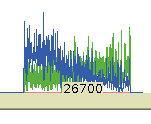
\includegraphics{energy_antigene.png}
	\caption{En vert les anticorps et en bleu les virus. Evolution du nombre d'entités en fonction du temps, en faisant varier le paramètre $\bf{energy\_antibody}$ de 20 à 100}
\end{figure}

\subsubsection{Les virus}
Ils disposent des même champs que les anticorps et de $\it{countdown_respawn}$ qui donne un temps limite moyen entre la reproduction d'un virus. Ce champs est rempli par le paramètre $\bf{antigene\_respawn}$.
\\
On peut changer le champ $\bf{epitope\_antigene}$ pour faire varier l'épitope du virus en présence.
\\
{ \color{red} $\bf{Attention!}$ on veillera à ne pas changer ce paramètre lorsque des virus sont présents.}

\newpage
\section{Le système immunitaire}
\subsection{Fonctionnement}
Le système immunitaire dispose de 3 fonctions :
\begin{enumerate}
	\item Envoyer 10 anticorps verts avec le paratope 1 
	\item Envoyer 10 anticorps jaunes avec le paratope 2
	\item Envoyer 10 anticorps bleus avec le paratope 3
\end{enumerate}
Tous les $\bf{immunity\_rapidity}$ ticks, on décide d'en utiliser une. La sélection se fait en calculant la qualité de réponse des anticorps, i.e. en déterminant le nombre de virus qu'ils ont réussi à tuer entre deux phases de décision. C'est pourquoi, il y a trois variables globales $\textbf{\textit{green\_killed}}$, $\textit{\textbf{yellow\_killed}}$ et $\textbf{\textit{pink\_killed}}$. On retient ensuite dans les matrices la réponse donnée par une fonction (= nombre de virus tués) en réponse à une attaque de virus, i.e. si elle est positive (virus tués) dans $\textbf{\textit{reward\_matrix}}$ ou négative (aucun virus tués) dans $\textbf{\textit{penalty\_matrix}}$, en incrémentant dans la bonne case. On mémorise égalemment dans $\textbf{\textit{specific\_matrix}}$ la quantité de fois qu'on a fait appel à une fonction donnée en présence d'un virus donné.
\\
Toutes ces données servent à calculer les ``concentrations'' des fonctions, i.e. quelle fonction utiliser en présence de quel virus. On peut faire une analogie entre notre système immunitaire et le système immunitaire réel selon l'hypothèse de Jerne.
\\
Les fonctions sont les anticorps réels, le nombre total de virus est un virus réel, et dans la réalité, le système sélectionne un anticorps par des mécanismes de simulations successives par les virus et entre les anticorps eux-mêmes. Ces mécanismes sont représentés dans notre modèle par les matrices qui retiennent l'efficacité des fonctions. Par conséquent l'anticorps en plus grande concentration sera celui qui lutte le mieux contre le virus.
\\
Pour calculer les concentrations des fonctions dans notre modèle (ce qui nous interesse ici puisque la fonction ayant une concentration maximale sera celle à envoyer), on utilise l'équation suivante:
\begin{equation}
	\frac{dA_i(t)}{dt} = \left(\alpha\cdot\frac{1}{N}\cdot\sum_{j=1}^{N}m_{ij}a_j(t)-\alpha \cdot \frac{1}{M}\cdot\sum_{k=1}^{M}m_{ik}a_k(t)+\beta m_i-k_i\right)\cdot a_i(t)
	\label{equation21}
\end{equation}
où : 
\begin{itemize}
	\item $a_i$ représente la concentration de la fonction $i$, les deux sommes de gauche représente respectivement la stimulation par les autres fonctions et l'inhibition
	\item $m_{ij}$ représente la stimulation de la fonction j par la fonction i. C'est ce terme précisément qui est calculé grace aux matrices précédentes.
	\item $m_i$ représente la stimulation directe par un virus (i.e. ce terme vaut 1 lorsque le système immunitaire appelle la fonction correspondante et 0 sinon)
	\item $k_i$ simule la mort naturelle des anticorps (peut être interprété comme un pourcentage de cellules qui meurent entre deux phases)
	\item $M$ est le nombre de fonction inhibant $i$ et $N$ le nombre de fonction stimulant $i$. Dans notre cas $M=N$, mais il est possible d'imaginer certains cas où les fonctions ne sont pas forcément toutes inhibitrices les unes des autres.
	\item $A_id$ est la concentration non normalisée  $a_i$, il faut alors le passer dans la fonction sigmoid : $f(x) = \frac{1}{1 + exp(0.5 - x)}$
\end{itemize}

Pour calculer $m_{ij}$ en présence du virus $k$ on applique la formule suivante \cite{ref}:
\begin{equation}
	m_{ij} = \frac {penalty\_matrix[i][k] + reward\_matrix[j][k]}{specific\_matrix[i][k] + specific\_matrix[j][k]}
\end{equation}
Plus clairement :
\begin{itemize}
	\item Au numérateur on somme la quantité de fois que la fonction $i$ n'a pas été efficace avec le virus k avec la quantité de fois que la fonction $j$ a été efficace avec le virus $k$.
	\item Au dénominateur, il y a le nombre de fois que chaque fonction a été appelée en présence du virus $k$.
\end{itemize}
	On comprend assez bien que si la fonction $i$ n'est pas efficace (grand nombre de pénalités), elle aura tendance à stimuler la fonction $j$, qu'elle soit efficace ou non, mais si elle l'est (important nombre de récompenses) elle aura une plus forte chance d'être appelé. L'ensemble constitue un poids entre 0 et 1 qui multipliera la concentration de la fonction $i$.
	
	\subsection{Paramètres liés au système immunitaire}
	On peut faire varier plusieurs paramètres.

\begin{itemize}
	\item $\bf{immunity\_rapidity}$ contrôle le temps entre deux phases de sélection de fonction. Ce paramètre permet essentiellement de réduire le nombre d'erreurs produites lors du contrôle de qualité d'une fonction (pénalité ou récompense). Plus il est grand, plus les anticorps ont le temps de tuer des virus s'ils le peuvent et de manifester à la fonction qu'ils sont positifs. En revanche, un délai trop court provoque des erreurs (affectation de pénalité à la fonction luttant contre le virus) car les anticorps n'auront pas le temps de tuer les virus. En fait, un délai trop long entraîne une convergence moins rapide vers la bonne fonction mais avec une très bonne précision, le délai court entraîne l'effet inverse.
	\item $\bf{natural\_death}$ est le terme $k_i$ de l'équation \ref{equation21}. Son rôle est relatif à la valeur de $\beta$. Si $\bf{natural\_death} << \beta$ alors, la concentration des fonctions ne fera que d'augmenter parce que les autres termes ne sont pas assez fort pour faire décroitre $a_i$. A l'inverse si $\bf{natural\_death} >> \beta$, alors les concentrations ne feront que descendre globalement, et on n'arrivera pas à sélectionner la bonne fonction. Dans les cas où $\bf{natural\_death} \simeq \beta$, on peut faire varier plus ou moins rapidement la vitesse de convergence.
	\item $\beta$ est modifiable avec le paramètre $\bf{beta}$
	\item $\alpha$ se modifie avec $\bf{alpha}$ et son rôle n'est pas explicitement déterminé.
\end{itemize}
\nocite{ref2}
\bibliographystyle{plain}
\bibliography{biblio}

\end{document}
